\section{Results}
\label{sec:results}

\begin{table*}[t]
\centering
\caption{RQ1 cost structure and the RQ3 validity regime, by family. Sample size
\emph{orders} cost in every family (Spearman $\rho>0.7$, with
\StudyReplicationICSE\ $0.879$--$0.943$, \StudyEnergy\ $0.710$--$0.996$,
\StudyLinux\ near-monotone), so the table reports where it nonetheless fails
as a \emph{budget}. $\Ratio$ is the median train-cost share divided by the count
share $n/|C|$ ($\Ratio{=}1$ is calibrated), and ``cost spread'' is per-configuration
heterogeneity ($p_{90}/p_{10}$ or CV). Regime: \emph{validated} (count
conclusions survive), \emph{warning} (the efficient set changes but few top
choices flip), \emph{changed} (the recommendation itself moves). %RQ2 change \emph{magnitudes} are in \Cref{tab:rq-metrics}.
}
\label{tab:decision-summary}
\footnotesize
\setlength{\tabcolsep}{4pt}
\renewcommand{\arraystretch}{1}
\begin{tabular}{p{0.12\linewidth} p{0.13\linewidth} p{0.22\linewidth} p{0.40\linewidth}}
\toprule
Family & Budget $\Ratio$ & Cost spread & Validity regime \& main lesson \\
\midrule
\StudyReplicationICSE & $0.80$--${\sim}1$ & $p_{90}/p_{10}=1.2$ (LLVM)--$47$ (lrzip, BerkeleyDBC) & Validated (LLVM, Polly, Dune, HIPAcc) to warning (7z, BerkeleyDBC). Published claims can flip. \\
\StudyReplicationICPE & ${\approx}1$ (aggregate) & strategy-biased: Henard $<$ $t$-wise & Changed under time-cost/size-target asymmetry. \\
\StudyEnergy & $0.17$--${\sim}1$ & $p_{90}/p_{10}=1.2$--$149$, CV $\le7.1$ (jump3r) & Spans tight/validated (PostgreSQL, LLVM) to heavy-tailed/changed (brotli, kanzi). Validity is per-system. \\
\StudyWorkload & $0.66$--$1.06$ & varies by workload & Changed in most contexts. The workload sets cost validity. \\
\StudyLCBench & $0.67$--$1.01$ & CV $0.60$--$2.25$ & Changed. The gap is not confined to configurable software. \\
\StudyLinux & $1.0$ (random)--$1.5$ (diversity) & CV $0.99$--$1.43$ & Changed every release. Scale and image-size cost expose strategy bias. \\
\bottomrule
\end{tabular}
\end{table*}

\subsection{RQ1: Sample Size Orders Cost, But Does Not Budget It}
\label{subsec:results-rq1}

\begin{figure}[t]
\centering
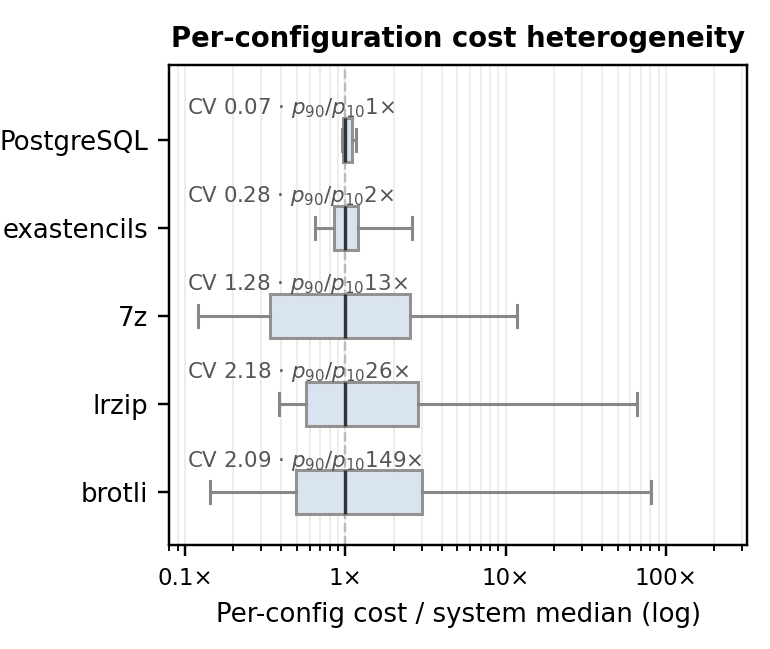
\includegraphics[width=0.88\columnwidth]{pic/results/fig_cost_distribution_regimes.png}
\caption{Per-configuration cost heterogeneity across energy systems: each box is
the per-config cost normalized by the system median (IQR box, min/max whiskers,
log scale), annotated with CV and $p_{90}/p_{10}$.}
\label{fig:distribution-regimes}
\end{figure}

\Cref{fig:distribution-regimes} illustrates the mechanism behind RQ1: how
strongly per-configuration costs vary within a system (CV and $p_{90}/p_{10}$
quantify the same spread). PostgreSQL is the validated extreme: costs are tight,
so sample count is a faithful budget proxy. As the distribution widens (7z,
lrzip, brotli) a fixed $n$ can spend wildly different measured budgets depending
on which configurations a strategy selects, which is what lets measured cost
re-order the sampler comparison.

Sample size is a useful ordering signal. In every family where we can test it,
larger samples are positively rank-correlated with measured cost.
This matters: count-based plots are not arbitrary, and $n$ remains a useful
common language for comparing sampling campaigns. In the
\StudyReplicationICSE revisit, Spearman correlation between sample size and
measured cost is high ($\rho=0.879$--$0.943$). The same ordering signal appears
in other families as well: \StudyEnergy remains positive even in its
hardest cases ($\rho=0.710$--$0.996$), and \StudyLinux is near monotone across
the six releases.

The failure is budget calibration. At fixed $n$, strategies can visit very
different cost regions: in the running example, five lrzip strategies all use
$n=16$ yet span a $16.5\times$ measured-cost gap for nearly identical MRE
(\Cref{fig:running-example}). Across families the cost spread ranges from benign
(LLVM $p_{90}/p_{10}=1.21$) to heavy-tailed (brotli $p_{90}/p_{10}=149$, lrzip and
BerkeleyDBC $\approx47$, jump3r CV $7.1$, Linux CV up to $1.4$,
\StudyLCBench CV up to $2.25$), with the \StudyEnergy family alone spanning both
extremes, and the
budget ratio drifts from calibrated to far below one (\StudyEnergy reaches
$\Ratio=0.17$, BerkeleyDBC $0.80$, workload and \StudyLCBench spanning
$0.66$--$1.06$).

This spread is strong enough to invert the size ordering itself. Within a single
strategy a larger sample almost never costs less ($<1\%$ of size pairs: cost is
monotone in a strategy's own $n$). \emph{Across} strategies it is common: a larger
sample drawn by a cheap sampler routinely undercuts a smaller sample drawn by a
costlier one. This cross-strategy reversal occurs in $11\%$ of \StudyEnergy\
comparisons and at least once in $79\%$ of its contexts, yet under the homogeneous
costs of the replication archives it is essentially absent ($\le 0.8\%$). The
count axis can thus not only mis-scale the budget but reverse it, and only where
costs are heavy-tailed, that is, where a few configurations are far more expensive
than the rest, the unsafe regime we analyze in \Cref{subsec:results-rq3}.

The x264 revisit explains why aggregate calibration is not enough. Its time
budgets look well calibrated when averaged over inputs, yet strategies are not
interchangeable: Henard-style samples tend to be cheaper, whereas $t$-wise
samples tend to be costlier. Thus a family can pass the coarse ``does $n$ order
cost?'' check and still fail the same-size, strategy-specific budget check that
matters for recommendations.


These three checks can disagree, and strategy bias, whether two same-$n$ samples
spend different budgets, is the mechanism behind most practical failures. On
Linux, random-like strategies stay close to the count budget while diversity costs
$1.24$--$1.52\times$ its count share, so an aggregate plot can look safe while a
specific strategy is not. \Cref{fig:running-example} is the sharpest local
instance: five strategies tied at $n{=}16$ yet separated by $16.5\times$ in
measured cost.

\rqfinding{Answer to RQ1}{Sample size is a useful ordering variable, but it is
not a calibrated budget. Across all families, larger samples usually cost more.
Nevertheless, same-size samples can differ by orders of magnitude in measured
cost, and across strategies a larger sample of a cheap sampler can be cheaper than
a smaller one of a costlier sampler ($11\%$ of \StudyEnergy\ comparisons), though
this is near-absent under homogeneous costs.}

\subsection{RQ2: Measured Cost Changes Strategy Assessment}
\label{subsec:results-rq2}

We read RQ2 through the three lenses of \Cref{sec:study_design}: the
cost-controlled Kruskal--Wallis (KW) sampler comparison (primary), the Pareto
choice set (robust, decision-level), and the top-$1$ flip (a narrow
illustration). The headline is the KW result. Each sampler enters at the largest predefined
sample affordable at a common measured budget (\Cref{sec:study_design}), and the
retrospective cheapest-error envelope, reported as a sensitivity check, agrees. Rerunning the replication studies' own
best-sampler test this way, instead of at a fixed sample size, the top group of
statistically
recommendable samplers changes in $8/21$ \StudyReplicationICSE comparisons
($38\%$), $28/51$ x264 comparisons ($55\%$), $56/112$ \StudyEnergy comparisons
($50\%$), $389/846$ \StudyWorkload contexts ($46\%$), and (outside configurable
software) $146/350$ \StudyLCBench datasets ($42\%$): $38$--$55\%$ across the five
non-Linux families. \StudyLinux is the extreme case rather than the exception:
even though its target \emph{is} the acquisition cost (\texttt{vmlinux} size),
strategy-level cost bias reshuffles the top group in all $30$ corrected
comparisons ($100\%$).

To check that these changes are not single-draw artifacts, we bootstrap the
membership change itself: resample each sampler's per-seed errors, recompute both
Dunn top groups ($B{=}1000$), and ask how often the change reproduces. It is
highly reproducible on the families that ground the published-verdict claim (all
x264 changes, $93\%$ on \StudyLinux, and $75\%$ on \StudyReplicationICSE), bbut
only a third to a half of the changes ($29$--$52\%$) reproduce on
\StudyEnergy/\StudyWorkload/\StudyLCBench, where the tied-best samplers are
near-ties (equal-budget MRE gaps of $0.2$--$2.0$pp). The recommendation-level
signal is sharper: the source study's own recommended sampler is \emph{evicted}
from the cost-controlled top group in $29$--$41\%$ of replication comparisons.
The omnibus KW remains significant in both views in $74$--$100\%$ of comparisons.
\Cref{tab:rq-metrics} collects the per-family numbers for both robust lenses.

\begin{table*}[t]
\centering
\caption{RQ2 across families: how often measured cost changes the conclusion
relative to sample count. \textbf{Kruskal--Wallis (KW)} reruns each study's own
best-sampler test at a fixed measured budget versus a fixed sample size.
\emph{Top-group~$\Delta$} is how often the Dunn/Holm set of statistically
tied-best samplers changes. \emph{Robust~$\Delta$} is the subset that reproduces in
$\ge95\%$ of seed-bootstrap resamples ($B{=}1000$). \emph{Evicted} is how often the
source study's own recommended sampler drops out of the cost-controlled top
group. \textbf{Pareto} gives how often the measured-cost efficient choice set
differs from the count one, reproducibly under the bootstrap
($p_{\text{differ}}\ge0.95$). \emph{Med.\ Jaccard} is the effect size (lower $=$
menus share fewer designs). The omnibus KW is significant in \emph{both} views in
$74$--$100\%$ of comparisons, and equal-budget MRE gaps on changed comparisons
are small ($0.2$--$3.9$pp). Comparison counts $N$ (KW/Pareto):
\StudyReplicationICSE\ $21/7$, x264 $51/17$, \StudyEnergy\ $112/56$,
\StudyWorkload\ $846/93$, \StudyLCBench\ $350/35$, \StudyLinux\ $30/6$. The
broader top-$1$ decision flip across cost weights ($32\%$, $538/1{,}666$, discussed
below) is a separate, weaker lens.}
\label{tab:rq-metrics}
\small
\setlength{\tabcolsep}{6pt}
\renewcommand{\arraystretch}{1.05}
\begin{tabular}{l ccc cc}
\toprule
& \multicolumn{3}{c}{Kruskal--Wallis sampler test} & \multicolumn{2}{c}{Pareto choice set} \\
\cmidrule(lr){2-4}\cmidrule(lr){5-6}
Family & top-group $\Delta$ & robust $\Delta$ & evicted & differs & med.\ Jaccard \\
\midrule
\StudyReplicationICSE\ (Kaltenecker~\cite{kaltenecker2019}, 7 systems) & $38\%$  & $29\%$ & $29\%$ & $86\%$  & $0.50$ \\
\StudyReplicationICPE\ (x264~\cite{pereira2020}, 17 inputs) & $55\%$  & $55\%$ & $41\%$ & $100\%$ & $0.33$ \\
\StudyEnergy\ (ICSE'23~\cite{weber2023twins}, 14 systems) & $50\%$  & $26\%$ & $17\%$ & $80\%$  & $0.65$ \\
\StudyWorkload\ (ICSE'23~\cite{muhlbauer2023workload}, 9 systems, 93 contexts) & $46\%$  & $21\%$ & $14\%$ & $73\%$  & $0.60$ \\
\StudyLCBench\ (LCBench~\cite{zimmer2021autopytorch}, 35 datasets) & $42\%$  & $12\%$ & $11\%$ & $89\%$  & $0.62$ \\
\StudyLinux\ (TuxKConfig~\cite{martin2022linux}, 6 releases) & $100\%$ & $93\%$ & $23\%$ & $100\%$ & $0.38$ \\
\midrule
Range                                & $38$--$100\%$ & $12$--$93\%$ & $11$--$41\%$ & $73$--$100\%$ & $0.33$--$0.65$ \\
\bottomrule
\end{tabular}
\end{table*}

This is a direct revisit of the replication studies' conclusions. Before
changing the cost axis we confirmed that our size-controlled replay reproduces
the source studies' fixed-$n$ verdicts: the size-view KW top groups
qualitatively match their reported outcomes (random a strong baseline across most
\StudyReplicationICSE systems, solver-based and $t$-wise competitive on x264), so
the changes reported below are attributable to the measured-cost axis rather than
a divergent replication. Kaltenecker
\etal\ \cite{kaltenecker2019} find distance-based samplers competitive at a fixed
sample size. At a fixed measured cost, diversified distance-based sampling falls
from best in $4$ comparisons to $1$, plain distance-based rises from $0$ to $2$,
and random stays dominant ($11$): \eg LLVM at the largest budget moves
\texttt{divDistBased}$\to$\texttt{random}, Polly
\texttt{solverBased}$\to$\texttt{random}. Pereira \etal\ \cite{pereira2020} show
x264 rankings shifting across inputs and targets. We add an orthogonal axis,
holding input and target fixed and changing only count\,$\to$\,measured cost:
\texttt{solverBased}, which selects expensive configurations, drops from best in
$12$ comparisons to $5$, while \texttt{divDistBased} rises from $7$ to $14$ (\eg
x264 input~$4$ at $t_1$ moves \texttt{solverBased}$\to$\texttt{divDistBased}). The
direction is consistent and mechanistic: at an equal budget an expensive sampler
cannot afford as large a sample, so it loses to cheaper samplers that buy more
data (see \Cref{subsec:results-rq3}). %\Cref{subsec:results-rq3} returns to why.

The choice-set lens is broader and the most robust. The measured-cost
Pareto-efficient set of strategy--budget combinations differs from the count-cost
set in almost every scenario, and the difference reproduces under the bootstrap
($p_{\text{differ}}\ge0.95$): in $45/56$ \StudyEnergy scenarios ($80\%$),
$68/93$ \StudyWorkload contexts ($73\%$), $31/35$ \StudyLCBench datasets
($89\%$), all $17$ x264 scenarios, and $6/7$ \StudyReplicationICSE systems, with
median Jaccard $0.60$--$0.65$. Even when the single best buy is stable, the menu
of efficient options a practitioner would compare is almost always different, and
that difference is not an artifact of one resampling. \Cref{fig:choiceset}
makes this concrete on the running example. On lrzip the count view's efficient
menu and the measured-cost menu share only $7$ of the $19$ designs either
certifies (Jaccard $0.37$): measured cost \emph{adds} $11$ designs the count view
discarded as ``too many samples'' (mostly large-$n$ \texttt{pilotCost} runs that
are cheap to measure) and drops $1$ it had kept. The efficient menu a
practitioner would compare is therefore not a refinement of the count one but a
genuinely different set. \StudyLinux, far from
being an exception, is the most extreme case. One might expect it to be safe: its
target \emph{is} the cost (\texttt{vmlinux} size), so $n$ tracks cost in
aggregate, yet with a full-feature learner the top group changes in all $30$
comparisons ($100\%$) and the choice set robustly differs on every release
($6/6$, median Jaccard $0.38$). The reason is exactly RQ1: even when count and
cost agree on average, strategy bias (diversity costs
$1.24$--$1.52\times$ its count share, active learning drifts) makes same-size
samples spend very different budgets, so the cost-controlled ranking still moves.
\Cref{tab:decision-summary} locates these changes by family.

\begin{figure}[t]
\centering
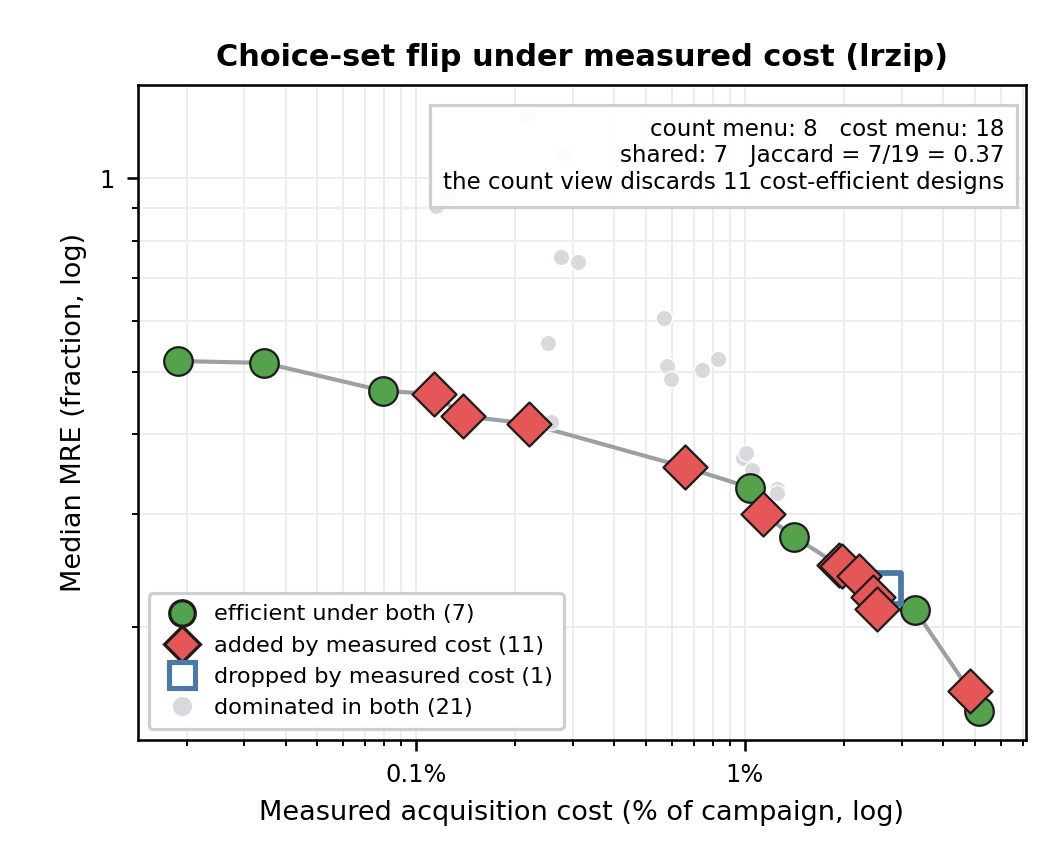
\includegraphics[width=0.9\columnwidth]{pic/results/choiceset_flip_lrzip.png}
\caption{The efficient choice set \emph{flips} under measured cost
(lrzip$\to$energy, the running example). Strategy--budget designs in the cost
decision space (lower-left better). Grey line is the measured-cost Pareto
frontier. The count and measured-cost menus ($8$ and $18$ designs) share only
$7$ (Jaccard $0.37$): measured cost adds $11$ (mostly cheap large-$n$
\texttt{pilotCost}) and drops $1$. The learner fits well ($0.15$ MRE), so this
is a real divergence, not an artifact.}
\label{fig:choiceset}
\end{figure}

The top-$1$ flip is the narrowest lens, and we report it as such. The single
best strategy--budget combination changes in $538/1{,}666$ context--weight
decisions ($32\%$). Most are near-ties in $J$, and the bootstrap-robust flips
($p_{\text{reproduce}}\ge0.95$) concentrate exactly where the KW and Pareto
lenses already move: where the target differs from the acquisition cost ($9$
robust x264 flips, all asymmetric) or cost is heavy-tailed (\StudyEnergy jump3r).
The flip corroborates the stronger lenses. It does not carry the claim alone. It
also underlines that the cost model is part of the experimental question: for
energy prediction the label is energy, but obtaining it requires running the
configuration, so execution time, not the target, is the natural acquisition
cost.

A changed verdict is not always ``the count winner was worse.'' Often it is more
accurate but costlier ($293/538$, $54\%$ of flips), so the question is whether
the accuracy gain is worth the budget. The remaining $188/538$ ($35\%$) are the
mirror case, cheaper but less accurate. ``Best at sample size $n$'' and ``best at
measured budget'' are simply different claims. The strict failures, the
$57/538$ ($11\%$) \emph{dominated} cases, are where no trade-off excuse exists:
a same-size or larger alternative is both cheaper and no less accurate, as in
\Cref{fig:running-example}. RQ2 therefore does not penalize accuracy. It asks
whether an accuracy advantage survives once the training-label resource is
charged.

\rqfinding{Answer to RQ2}{Measured cost changes sampling conclusions on their own
terms. At a fixed measured budget, the replication studies' own Kruskal--Wallis
test re-draws the set of statistically tied-best samplers in $38$--$55\%$ of
comparisons (all of them on Linux), and the change is most reproducible exactly
where the published verdicts live (every x264 change, $93\%$ on Linux, $75\%$ on
\StudyReplicationICSE). Sharper still, the source study's recommended sampler is
\emph{evicted} from the top group in $29$--$41\%$ of replication comparisons, and
the Pareto-efficient choice set robustly differs in $73$--$100\%$ of scenarios.
The single-winner flip agrees but is a fragile near-tie.}

\subsection{RQ3: Validity Conditions}
\label{subsec:results-rq3}

The count proxy is most defensible when per-configuration costs are tight, when
the target and acquisition resource are the same, and when the strategy does
not bias itself toward costly regions. It is most fragile when costs are
heavy-tailed, when target and cost differ, when workload or dataset changes the
cost distribution, or when the strategy explicitly seeks diversity or uncertain
regions.

\paragraph*{Why cost moves the verdict.} The mechanism is RQ1 propagating into
the sampler comparison. For a fixed strategy and size, MRE is a fixed number, so
re-pricing cost cannot change it directly. What changes is the cost-controlled
comparison: at an equal measured budget a cheap sampler affords a larger sample
(lower error) and an expensive one affords fewer (higher error), because the
size$\to$cost map is strategy-dependent (RQ1). Re-indexing operating points by
cost is thus a non-uniform permutation, not a rescaling, so the accuracy ranking
need not be preserved: \texttt{solverBased}, which selects expensive
configurations, repeatedly loses to \texttt{random} and \texttt{divDistBased} at
equal budget. The count proxy therefore fails precisely when per-configuration
costs are heterogeneous or the target differs from the paid resource.

Four recurring mechanisms explain why the proxy fails, in increasing severity:
(i)~a same-size choice can carry a large measured-cost gap (the count axis has
lost budget information, though the preferred sampler may be unchanged). (ii)~Two
choices can have similar MRE but very different cost (wasted budget without an
accuracy payoff). (iii)~A larger sample can be cheaper in measured time
(contradicting the monotone more-configurations-cost-more intuition).
(iv)~Classic same-budget configurable-system strategies can separate once
measured cost is charged: the case closest to prior sampling papers, showing
that even familiar fixed-nominal-budget comparisons can change under
heterogeneous cost. These are representative patterns, not exhaustive
evidence (\Cref{tab:rq-metrics} and the family paragraphs give that).

\begin{figure}[t]
\centering
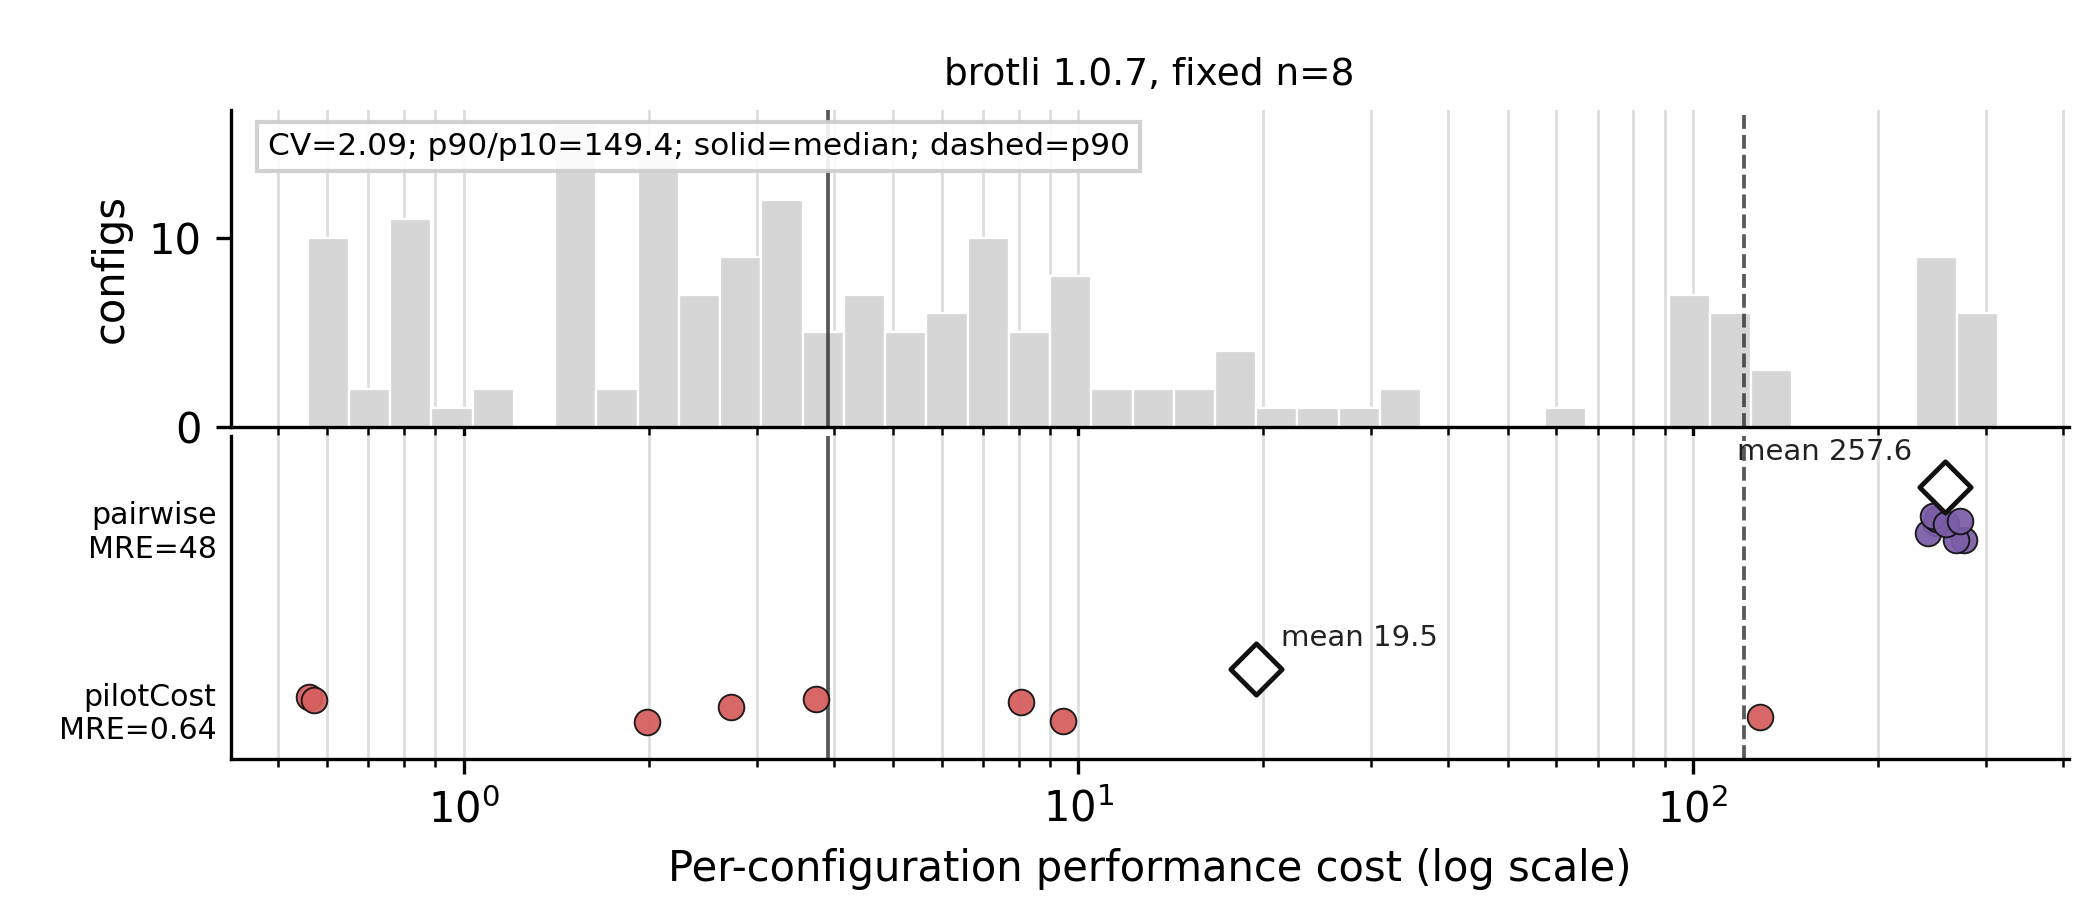
\includegraphics[width=\columnwidth]{pic/results/twins_brotli_fixed_n8_with_distribution.png}
\caption{Distribution-aware RQ3 example (brotli, fixed $n{=}8$). Top: the full
per-configuration performance-cost distribution. Bottom: where \texttt{pairwise}
and a representative \texttt{pilotCost} sample fall (circles = selected configs,
diamonds = sample mean, labels = energy MRE). \texttt{pairwise} selects the
expensive tail. \texttt{pilotCost} stays in the cheap bulk.}
\label{fig:brotli-distribution}
\end{figure}

\Cref{fig:brotli-distribution} opens one of these patterns by showing both the
strategy outcomes and the underlying cost distribution. All strategies use the
same $n=8$ count budget, yet pairwise selects eight configurations above the
full campaign's $p_{90}$ performance cost. Its mean selected cost is $257.6$,
it spends $31.2\%$ of the full measured budget, and its energy-prediction MRE is
$48.0$ (\ie predictions off by about $48\times$), because its expensive-tail
sample extrapolates poorly to the rest of the space. Pilot-cost is not an oracle for the cheapest configurations: in the
representative sample shown, its initial pilot includes one expensive point above
$p_{90}$ (and the pilot's own measurement cost is charged in $\TrainCost$, so the
strategy pays for the configurations it probes). Its cost-guided fill still places
the other seven selections in the low-to-mid-cost bulk, yielding mean selected
cost $19.5$, $2.36\%$ of the full measured budget, and MRE $0.64$ for that sample.

\paragraph*{Cross-RQ synthesis.}
The families fall into three practical regimes. In the \emph{validated-transfer}
regime, count-based conclusions survive the measured-cost check. LLVM, Polly,
Dune, HIPAcc, PostgreSQL, and x264 time/time are the main examples: costs are
tight enough, or the strategies are cost-unaware enough, that replacing count by
measured cost does not change the top recommendation. In the \emph{warning}
regime, the top recommendation mostly survives but the efficient choice set
changes. 7Z and BerkeleyDBC fit this pattern: a reader who only wants the single
winner may reach the same conclusion, but a reader comparing trade-offs would
miss measured-cost-efficient alternatives. In the \emph{changed-assessment}
regime, measured cost changes the recommendation itself. lrzip, the asymmetric
x264 time-cost/size-target scenario, heavy-tailed performance--energy systems,
many workload contexts, most \StudyLCBench datasets, and every Linux release
fall here. The scientific message is not that one sampler dominates in all
settings. It is that the validity of the count proxy is an empirical property of
the dataset, workload, cost dimension, and strategy panel. As a proof of concept
that these conditions are not merely narrative, a simple classifier over the RQ1
diagnostics ($p_{90}/p_{10}$, per-strategy $\Ratio$ spread, and target--cost
asymmetry) identifies where measured cost \emph{materially} changes the
recommended sampler. Across the $167$ contexts (each a system, input, workload,
dataset, or release), the ones it ranks high-risk change in $85\%$ of cases versus
$32\%$ for the rest (five-fold cross-validated, AUC $\approx0.78$, driven mainly by
cost spread)~\cite{artifact}.

\rqfinding{Answer to RQ3}{Sample size is safest as a cost proxy when
per-configuration costs are tight, the target and bottleneck resource coincide,
and strategies are cost-unaware. It is unsafe when costs are heavy-tailed,
target and acquisition cost differ, workload or dataset changes the cost
distribution, or the strategy deliberately searches unusual, diverse, or
uncertain regions.}
